\documentclass[1p]{elsarticle_modified}
%\bibliographystyle{elsarticle-num}

%\usepackage[colorlinks]{hyperref}
%\usepackage{abbrmath_seonhwa} %\Abb, \Ascr, \Acal ,\Abf, \Afrak
\usepackage{amsfonts}
\usepackage{amssymb}
\usepackage{amsmath}
\usepackage{amsthm}
\usepackage{scalefnt}
\usepackage{amsbsy}
\usepackage{kotex}
\usepackage{caption}
\usepackage{subfig}
\usepackage{color}
\usepackage{graphicx}
\usepackage{xcolor} %% white, black, red, green, blue, cyan, magenta, yellow
\usepackage{float}
\usepackage{setspace}
\usepackage{hyperref}

\usepackage{tikz}
\usetikzlibrary{arrows}

\usepackage{multirow}
\usepackage{array} % fixed length table
\usepackage{hhline}

%%%%%%%%%%%%%%%%%%%%%
\makeatletter
\renewcommand*\env@matrix[1][\arraystretch]{%
	\edef\arraystretch{#1}%
	\hskip -\arraycolsep
	\let\@ifnextchar\new@ifnextchar
	\array{*\c@MaxMatrixCols c}}
\makeatother %https://tex.stackexchange.com/questions/14071/how-can-i-increase-the-line-spacing-in-a-matrix
%%%%%%%%%%%%%%%

\usepackage[normalem]{ulem}

\newcommand{\msout}[1]{\ifmmode\text{\sout{\ensuremath{#1}}}\else\sout{#1}\fi}
%SOURCE: \msout is \stkout macro in https://tex.stackexchange.com/questions/20609/strikeout-in-math-mode

\newcommand{\cancel}[1]{
	\ifmmode
	{\color{red}\msout{#1}}
	\else
	{\color{red}\sout{#1}}
	\fi
}

\newcommand{\add}[1]{
	{\color{blue}\uwave{#1}}
}

\newcommand{\replace}[2]{
	\ifmmode
	{\color{red}\msout{#1}}{\color{blue}\uwave{#2}}
	\else
	{\color{red}\sout{#1}}{\color{blue}\uwave{#2}}
	\fi
}

\newcommand{\Sol}{\mathcal{S}} %segment
\newcommand{\D}{D} %diagram
\newcommand{\A}{\mathcal{A}} %arc


%%%%%%%%%%%%%%%%%%%%%%%%%%%%%5 test

\def\sl{\operatorname{\textup{SL}}(2,\Cbb)}
\def\psl{\operatorname{\textup{PSL}}(2,\Cbb)}
\def\quan{\mkern 1mu \triangleright \mkern 1mu}

\theoremstyle{definition}
\newtheorem{thm}{Theorem}[section]
\newtheorem{prop}[thm]{Proposition}
\newtheorem{lem}[thm]{Lemma}
\newtheorem{ques}[thm]{Question}
\newtheorem{cor}[thm]{Corollary}
\newtheorem{defn}[thm]{Definition}
\newtheorem{exam}[thm]{Example}
\newtheorem{rmk}[thm]{Remark}
\newtheorem{alg}[thm]{Algorithm}

\newcommand{\I}{\sqrt{-1}}
\begin{document}

%\begin{frontmatter}
%
%\title{Boundary parabolic representations of knots up to 8 crossings}
%
%%% Group authors per affiliation:
%\author{Yunhi Cho} 
%\address{Department of Mathematics, University of Seoul, Seoul, Korea}
%\ead{yhcho@uos.ac.kr}
%
%
%\author{Seonhwa Kim} %\fnref{s_kim}}
%\address{Center for Geometry and Physics, Institute for Basic Science, Pohang, 37673, Korea}
%\ead{ryeona17@ibs.re.kr}
%
%\author{Hyuk Kim}
%\address{Department of Mathematical Sciences, Seoul National University, Seoul 08826, Korea}
%\ead{hyukkim@snu.ac.kr}
%
%\author{Seokbeom Yoon}
%\address{Department of Mathematical Sciences, Seoul National University, Seoul, 08826,  Korea}
%\ead{sbyoon15@snu.ac.kr}
%
%\begin{abstract}
%We find all boundary parabolic representation of knots up to 8 crossings.
%
%\end{abstract}
%\begin{keyword}
%    \MSC[2010] 57M25 
%\end{keyword}
%
%\end{frontmatter}

%\linenumbers
%\tableofcontents
%
\newcommand\colored[1]{\textcolor{white}{\rule[-0.35ex]{0.8em}{1.4ex}}\kern-0.8em\color{red} #1}%
%\newcommand\colored[1]{\textcolor{white}{ #1}\kern-2.17ex	\textcolor{white}{ #1}\kern-1.81ex	\textcolor{white}{ #1}\kern-2.15ex\color{red}#1	}

{\Large $\underline{12n_{0707}~(K12n_{0707})}$}

\setlength{\tabcolsep}{10pt}
\renewcommand{\arraystretch}{1.6}
\vspace{1cm}\begin{tabular}{m{100pt}>{\centering\arraybackslash}m{274pt}}
\multirow{5}{120pt}{
	\centering
	\includegraphics[width=112pt]{../../../GIT/diagram.site/Diagrams/png/2796_12n_0707.png}\\
\ \ \ A knot diagram\footnotemark}&
\allowdisplaybreaks
\textbf{Linearized knot diagam} \\
\cline{2-2}
 &
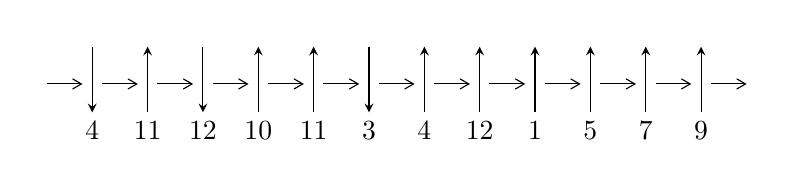
\begin{tikzpicture}[x=20pt, y=17pt]
	% nodes
	\node (C0) at (0, 0) {};
	\node (C1) at (1, 0) {};
	\node (C1U) at (1, +1) {};
	\node (C1D) at (1, -1) {4};

	\node (C2) at (2, 0) {};
	\node (C2U) at (2, +1) {};
	\node (C2D) at (2, -1) {11};

	\node (C3) at (3, 0) {};
	\node (C3U) at (3, +1) {};
	\node (C3D) at (3, -1) {12};

	\node (C4) at (4, 0) {};
	\node (C4U) at (4, +1) {};
	\node (C4D) at (4, -1) {10};

	\node (C5) at (5, 0) {};
	\node (C5U) at (5, +1) {};
	\node (C5D) at (5, -1) {11};

	\node (C6) at (6, 0) {};
	\node (C6U) at (6, +1) {};
	\node (C6D) at (6, -1) {3};

	\node (C7) at (7, 0) {};
	\node (C7U) at (7, +1) {};
	\node (C7D) at (7, -1) {4};

	\node (C8) at (8, 0) {};
	\node (C8U) at (8, +1) {};
	\node (C8D) at (8, -1) {12};

	\node (C9) at (9, 0) {};
	\node (C9U) at (9, +1) {};
	\node (C9D) at (9, -1) {1};

	\node (C10) at (10, 0) {};
	\node (C10U) at (10, +1) {};
	\node (C10D) at (10, -1) {5};

	\node (C11) at (11, 0) {};
	\node (C11U) at (11, +1) {};
	\node (C11D) at (11, -1) {7};

	\node (C12) at (12, 0) {};
	\node (C12U) at (12, +1) {};
	\node (C12D) at (12, -1) {9};
	\node (C13) at (13, 0) {};

	% arrows
	\draw[->,>={angle 60}]
	(C0) edge (C1) (C1) edge (C2) (C2) edge (C3) (C3) edge (C4) (C4) edge (C5) (C5) edge (C6) (C6) edge (C7) (C7) edge (C8) (C8) edge (C9) (C9) edge (C10) (C10) edge (C11) (C11) edge (C12) (C12) edge (C13) ;	\draw[->,>=stealth]
	(C1U) edge (C1D) (C2D) edge (C2U) (C3U) edge (C3D) (C4D) edge (C4U) (C5D) edge (C5U) (C6U) edge (C6D) (C7D) edge (C7U) (C8D) edge (C8U) (C9D) edge (C9U) (C10D) edge (C10U) (C11D) edge (C11U) (C12D) edge (C12U) ;
	\end{tikzpicture} \\
\hhline{~~} \\& 
\textbf{Solving Sequence} \\ \cline{2-2} 
 &
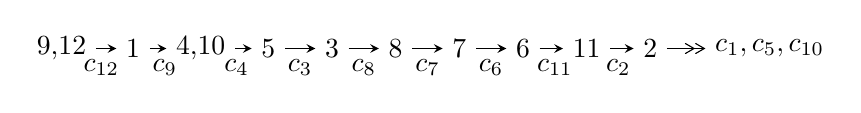
\begin{tikzpicture}[x=23pt, y=7pt]
	% node
	\node (A0) at (-1/8, 0) {9,12};
	\node (A1) at (1, 0) {1};
	\node (A2) at (33/16, 0) {4,10};
	\node (A3) at (25/8, 0) {5};
	\node (A4) at (33/8, 0) {3};
	\node (A5) at (41/8, 0) {8};
	\node (A6) at (49/8, 0) {7};
	\node (A7) at (57/8, 0) {6};
	\node (A8) at (65/8, 0) {11};
	\node (A9) at (73/8, 0) {2};
	\node (C1) at (1/2, -1) {$c_{12}$};
	\node (C2) at (3/2, -1) {$c_{9}$};
	\node (C3) at (21/8, -1) {$c_{4}$};
	\node (C4) at (29/8, -1) {$c_{3}$};
	\node (C5) at (37/8, -1) {$c_{8}$};
	\node (C6) at (45/8, -1) {$c_{7}$};
	\node (C7) at (53/8, -1) {$c_{6}$};
	\node (C8) at (61/8, -1) {$c_{11}$};
	\node (C9) at (69/8, -1) {$c_{2}$};
	\node (A10) at (11, 0) {$c_{1},c_{5},c_{10}$};

	% edge
	\draw[->,>=stealth]	
	(A0) edge (A1) (A1) edge (A2) (A2) edge (A3) (A3) edge (A4) (A4) edge (A5) (A5) edge (A6) (A6) edge (A7) (A7) edge (A8) (A8) edge (A9) ;
	\draw[->>,>={angle 60}]	
	(A9) edge (A10);
\end{tikzpicture} \\ 

\end{tabular} \\

\footnotetext{
The image of knot diagram is generated by the software ``\textbf{Draw programme}" developed by Andrew Bartholomew(\url{http://www.layer8.co.uk/maths/draw/index.htm\#Running-draw}), where we modified some parts for our purpose(\url{https://github.com/CATsTAILs/LinksPainter}).
}\phantom \\ \newline 
\centering \textbf{Ideals for irreducible components\footnotemark of $X_{\text{par}}$} 
 
\begin{align*}
I^u_{1}&=\langle 
-114 u^{14}-108 u^{13}+\cdots+299 b-79,\;310 u^{14}+215 u^{13}+\cdots+299 a-593,\\
\phantom{I^u_{1}}&\phantom{= \langle  }u^{15}-8 u^{13}+25 u^{11}-33 u^9+2 u^7- u^6+37 u^5+2 u^4-27 u^3- u^2+u+1\rangle \\
I^u_{2}&=\langle 
1.65560\times10^{32} u^{39}+3.59685\times10^{32} u^{38}+\cdots+2.03419\times10^{33} b+3.23849\times10^{33},\\
\phantom{I^u_{2}}&\phantom{= \langle  }-2.30658\times10^{33} u^{39}-2.80492\times10^{33} u^{38}+\cdots+1.42393\times10^{34} a-3.27516\times10^{34},\;u^{40}- u^{39}+\cdots+2 u-7\rangle \\
I^u_{3}&=\langle 
u^3+b-2 u,\;u^4- u^3-2 u^2+a+u,\;u^5-3 u^3+2 u-1\rangle \\
I^u_{4}&=\langle 
u^7-4 u^5- u^4+3 u^3+3 u^2+b+u-1,\;-3 u^7+14 u^5+2 u^4-17 u^3-7 u^2+a+4 u+6,\\
\phantom{I^u_{4}}&\phantom{= \langle  }u^8-5 u^6- u^5+7 u^4+4 u^3-2 u^2-4 u-1\rangle \\
\\
\end{align*}
\raggedright * 4 irreducible components of $\dim_{\mathbb{C}}=0$, with total 68 representations.\\
\footnotetext{All coefficients of polynomials are rational numbers. But the coefficients are sometimes approximated in decimal forms when there is not enough margin.}
\newpage
\renewcommand{\arraystretch}{1}
\centering \section*{I. $I^u_{1}= \langle -114 u^{14}-108 u^{13}+\cdots+299 b-79,\;310 u^{14}+215 u^{13}+\cdots+299 a-593,\;u^{15}-8 u^{13}+\cdots+u+1 \rangle$}
\flushleft \textbf{(i) Arc colorings}\\
\begin{tabular}{m{7pt} m{180pt} m{7pt} m{180pt} }
\flushright $a_{9}=$&$\begin{pmatrix}0\\u\end{pmatrix}$ \\
\flushright $a_{12}=$&$\begin{pmatrix}1\\0\end{pmatrix}$ \\
\flushright $a_{1}=$&$\begin{pmatrix}1\\- u^2\end{pmatrix}$ \\
\flushright $a_{4}=$&$\begin{pmatrix}-1.03679 u^{14}-0.719064 u^{13}+\cdots-0.645485 u+1.98328\\0.381271 u^{14}+0.361204 u^{13}+\cdots-2.40134 u+0.264214\end{pmatrix}$ \\
\flushright $a_{10}=$&$\begin{pmatrix}u\\- u^3+u\end{pmatrix}$ \\
\flushright $a_{5}=$&$\begin{pmatrix}-1.03679 u^{14}-0.719064 u^{13}+\cdots-0.645485 u+1.98328\\0.381271 u^{14}+0.361204 u^{13}+\cdots-2.40134 u+0.264214\end{pmatrix}$ \\
\flushright $a_{3}=$&$\begin{pmatrix}-0.655518 u^{14}-0.357860 u^{13}+\cdots-3.04682 u+2.24749\\0.381271 u^{14}+0.361204 u^{13}+\cdots-2.40134 u+0.264214\end{pmatrix}$ \\
\flushright $a_{8}=$&$\begin{pmatrix}- u\\u\end{pmatrix}$ \\
\flushright $a_{7}=$&$\begin{pmatrix}-0.277592 u^{14}+0.210702 u^{13}+\cdots-4.23411 u-0.762542\\-0.571906 u^{14}-0.541806 u^{13}+\cdots+0.602007 u+0.103679\end{pmatrix}$ \\
\flushright $a_{6}=$&$\begin{pmatrix}-0.381271 u^{14}-0.361204 u^{13}+\cdots+2.40134 u-1.26421\\0.224080 u^{14}+0.107023 u^{13}+\cdots+1.65886 u-0.625418\end{pmatrix}$ \\
\flushright $a_{11}=$&$\begin{pmatrix}-0.719064 u^{14}-1.41806 u^{13}+\cdots+4.02007 u+1.03679\\0.361204 u^{14}+0.605351 u^{13}+\cdots+0.882943 u-0.381271\end{pmatrix}$ \\
\flushright $a_{2}=$&$\begin{pmatrix}-0.625418 u^{14}-0.224080 u^{13}+\cdots-2.97324 u+1.71572\\0.518395 u^{14}+0.859532 u^{13}+\cdots-3.17726 u-0.491639\end{pmatrix}$\\&\end{tabular}
\flushleft \textbf{(ii) Obstruction class $= -1$}\\~\\
\flushleft \textbf{(iii) Cusp Shapes $= -\frac{1039}{299} u^{14}-\frac{465}{299} u^{13}+\cdots+\frac{3706}{299} u+\frac{1512}{299}$}\\~\\
\newpage\renewcommand{\arraystretch}{1}
\flushleft \textbf{(iv) u-Polynomials at the component}\newline \\
\begin{tabular}{m{50pt}|m{274pt}}
Crossings & \hspace{64pt}u-Polynomials at each crossing \\
\hline $$\begin{aligned}c_{1}\end{aligned}$$&$\begin{aligned}
&u^{15}-12 u^{14}+\cdots+352 u-16
\end{aligned}$\\
\hline $$\begin{aligned}c_{2},c_{7}\end{aligned}$$&$\begin{aligned}
&u^{15}- u^{14}+\cdots-9 u+1
\end{aligned}$\\
\hline $$\begin{aligned}c_{3},c_{6}\end{aligned}$$&$\begin{aligned}
&u^{15}-6 u^{13}+\cdots-2 u+1
\end{aligned}$\\
\hline $$\begin{aligned}c_{4},c_{5},c_{8}\\c_{9},c_{10},c_{12}\end{aligned}$$&$\begin{aligned}
&u^{15}-8 u^{13}+25 u^{11}-33 u^9+2 u^7- u^6+37 u^5+2 u^4-27 u^3- u^2+u+1
\end{aligned}$\\
\hline $$\begin{aligned}c_{11}\end{aligned}$$&$\begin{aligned}
&u^{15}+8 u^{14}+\cdots+2 u-4
\end{aligned}$\\
\hline
\end{tabular}\\~\\
\newpage\renewcommand{\arraystretch}{1}
\flushleft \textbf{(v) Riley Polynomials at the component}\newline \\
\begin{tabular}{m{50pt}|m{274pt}}
Crossings & \hspace{64pt}Riley Polynomials at each crossing \\
\hline $$\begin{aligned}c_{1}\end{aligned}$$&$\begin{aligned}
&y^{15}-2 y^{14}+\cdots+81824 y-256
\end{aligned}$\\
\hline $$\begin{aligned}c_{2},c_{7}\end{aligned}$$&$\begin{aligned}
&y^{15}+15 y^{14}+\cdots+13 y-1
\end{aligned}$\\
\hline $$\begin{aligned}c_{3},c_{6}\end{aligned}$$&$\begin{aligned}
&y^{15}-12 y^{14}+\cdots+38 y-1
\end{aligned}$\\
\hline $$\begin{aligned}c_{4},c_{5},c_{8}\\c_{9},c_{10},c_{12}\end{aligned}$$&$\begin{aligned}
&y^{15}-16 y^{14}+\cdots+3 y-1
\end{aligned}$\\
\hline $$\begin{aligned}c_{11}\end{aligned}$$&$\begin{aligned}
&y^{15}-2 y^{14}+\cdots+332 y-16
\end{aligned}$\\
\hline
\end{tabular}\\~\\
\newpage\flushleft \textbf{(vi) Complex Volumes and Cusp Shapes}
$$\begin{array}{c|c|c}  
\text{Solutions to }I^u_{1}& \I (\text{vol} + \sqrt{-1}CS) & \text{Cusp shape}\\
 \hline 
\begin{aligned}
u &= \phantom{-}0.012566 + 0.990836 I \\
a &= -0.211019 + 0.142592 I \\
b &= -1.41460 + 0.28782 I\end{aligned}
 & -8.15802 + 4.15828 I & \phantom{-}1.85862 - 2.84983 I \\ \hline\begin{aligned}
u &= \phantom{-}0.012566 - 0.990836 I \\
a &= -0.211019 - 0.142592 I \\
b &= -1.41460 - 0.28782 I\end{aligned}
 & -8.15802 - 4.15828 I & \phantom{-}1.85862 + 2.84983 I \\ \hline\begin{aligned}
u &= \phantom{-}1.169430 + 0.063677 I \\
a &= \phantom{-}0.64821 + 2.11508 I \\
b &= -0.920632 - 0.865411 I\end{aligned}
 & \phantom{-}3.87319 - 2.68365 I & \phantom{-}10.95805 + 3.07423 I \\ \hline\begin{aligned}
u &= \phantom{-}1.169430 - 0.063677 I \\
a &= \phantom{-}0.64821 - 2.11508 I \\
b &= -0.920632 + 0.865411 I\end{aligned}
 & \phantom{-}3.87319 + 2.68365 I & \phantom{-}10.95805 - 3.07423 I \\ \hline\begin{aligned}
u &= -1.246380 + 0.258821 I \\
a &= \phantom{-}0.538407 - 0.957075 I \\
b &= -0.644440 + 0.812972 I\end{aligned}
 & \phantom{-}6.72141 - 1.91087 I & \phantom{-}13.27233 + 1.33121 I \\ \hline\begin{aligned}
u &= -1.246380 - 0.258821 I \\
a &= \phantom{-}0.538407 + 0.957075 I \\
b &= -0.644440 - 0.812972 I\end{aligned}
 & \phantom{-}6.72141 + 1.91087 I & \phantom{-}13.27233 - 1.33121 I \\ \hline\begin{aligned}
u &= -1.43453\phantom{ +0.000000I} \\
a &= \phantom{-}0.152509\phantom{ +0.000000I} \\
b &= -1.16134\phantom{ +0.000000I}\end{aligned}
 & \phantom{-}8.30719\phantom{ +0.000000I} & \phantom{-}10.1930\phantom{ +0.000000I} \\ \hline\begin{aligned}
u &= -1.45450 + 0.38452 I \\
a &= -0.85460 - 1.15788 I \\
b &= \phantom{-}1.122180 + 0.164567 I\end{aligned}
 & \phantom{-}1.22162 - 5.77031 I & \phantom{-}7.48274 + 3.55671 I \\ \hline\begin{aligned}
u &= -1.45450 - 0.38452 I \\
a &= -0.85460 + 1.15788 I \\
b &= \phantom{-}1.122180 - 0.164567 I\end{aligned}
 & \phantom{-}1.22162 + 5.77031 I & \phantom{-}7.48274 - 3.55671 I \\ \hline\begin{aligned}
u &= \phantom{-}1.45202 + 0.46014 I \\
a &= -0.49137 + 1.50243 I \\
b &= \phantom{-}1.44823 - 0.69051 I\end{aligned}
 & \phantom{-}1.2931 + 14.7754 I & \phantom{-}9.28197 - 7.69335 I\\
 \hline 
 \end{array}$$\newpage$$\begin{array}{c|c|c}  
\text{Solutions to }I^u_{1}& \I (\text{vol} + \sqrt{-1}CS) & \text{Cusp shape}\\
 \hline 
\begin{aligned}
u &= \phantom{-}1.45202 - 0.46014 I \\
a &= -0.49137 - 1.50243 I \\
b &= \phantom{-}1.44823 + 0.69051 I\end{aligned}
 & \phantom{-}1.2931 - 14.7754 I & \phantom{-}9.28197 + 7.69335 I \\ \hline\begin{aligned}
u &= \phantom{-}1.54559\phantom{ +0.000000I} \\
a &= -0.962536\phantom{ +0.000000I} \\
b &= \phantom{-}0.336815\phantom{ +0.000000I}\end{aligned}
 & \phantom{-}14.2541\phantom{ +0.000000I} & \phantom{-}21.6380\phantom{ +0.000000I} \\ \hline\begin{aligned}
u &= \phantom{-}0.391264\phantom{ +0.000000I} \\
a &= \phantom{-}0.943881\phantom{ +0.000000I} \\
b &= -0.200615\phantom{ +0.000000I}\end{aligned}
 & \phantom{-}0.640876\phantom{ +0.000000I} & \phantom{-}15.5990\phantom{ +0.000000I} \\ \hline\begin{aligned}
u &= -0.184294 + 0.258098 I \\
a &= \phantom{-}1.80344 - 0.62550 I \\
b &= \phantom{-}0.921833 - 0.474362 I\end{aligned}
 & -1.74796 + 1.39281 I & -0.06858 - 4.56854 I \\ \hline\begin{aligned}
u &= -0.184294 - 0.258098 I \\
a &= \phantom{-}1.80344 + 0.62550 I \\
b &= \phantom{-}0.921833 + 0.474362 I\end{aligned}
 & -1.74796 - 1.39281 I & -0.06858 + 4.56854 I\\
 \hline 
 \end{array}$$\newpage\newpage\renewcommand{\arraystretch}{1}
\centering \section*{II. $I^u_{2}= \langle 1.66\times10^{32} u^{39}+3.60\times10^{32} u^{38}+\cdots+2.03\times10^{33} b+3.24\times10^{33},\;-2.31\times10^{33} u^{39}-2.80\times10^{33} u^{38}+\cdots+1.42\times10^{34} a-3.28\times10^{34},\;u^{40}- u^{39}+\cdots+2 u-7 \rangle$}
\flushleft \textbf{(i) Arc colorings}\\
\begin{tabular}{m{7pt} m{180pt} m{7pt} m{180pt} }
\flushright $a_{9}=$&$\begin{pmatrix}0\\u\end{pmatrix}$ \\
\flushright $a_{12}=$&$\begin{pmatrix}1\\0\end{pmatrix}$ \\
\flushright $a_{1}=$&$\begin{pmatrix}1\\- u^2\end{pmatrix}$ \\
\flushright $a_{4}=$&$\begin{pmatrix}0.161987 u^{39}+0.196985 u^{38}+\cdots-3.44398 u+2.30009\\-0.0813887 u^{39}-0.176820 u^{38}+\cdots-0.179851 u-1.59203\end{pmatrix}$ \\
\flushright $a_{10}=$&$\begin{pmatrix}u\\- u^3+u\end{pmatrix}$ \\
\flushright $a_{5}=$&$\begin{pmatrix}-0.163111 u^{39}+0.121091 u^{38}+\cdots-2.45449 u-0.157285\\0.0118001 u^{39}-0.161041 u^{38}+\cdots+2.28334 u-1.24246\end{pmatrix}$ \\
\flushright $a_{3}=$&$\begin{pmatrix}0.0805980 u^{39}+0.0201647 u^{38}+\cdots-3.62383 u+0.708055\\-0.0813887 u^{39}-0.176820 u^{38}+\cdots-0.179851 u-1.59203\end{pmatrix}$ \\
\flushright $a_{8}=$&$\begin{pmatrix}- u\\u\end{pmatrix}$ \\
\flushright $a_{7}=$&$\begin{pmatrix}-0.686240 u^{39}+0.165773 u^{38}+\cdots-8.36308 u-2.07268\\-0.124536 u^{39}-0.0137535 u^{38}+\cdots+3.30823 u-1.30076\end{pmatrix}$ \\
\flushright $a_{6}=$&$\begin{pmatrix}-0.264297 u^{39}+0.208180 u^{38}+\cdots-8.40248 u+1.25906\\-0.0917954 u^{39}-0.149519 u^{38}+\cdots+1.01878 u-1.41043\end{pmatrix}$ \\
\flushright $a_{11}=$&$\begin{pmatrix}0.362372 u^{39}-0.240314 u^{38}+\cdots+6.14938 u-0.500854\\0.0561169 u^{39}+0.187756 u^{38}+\cdots-1.78765 u+1.85008\end{pmatrix}$ \\
\flushright $a_{2}=$&$\begin{pmatrix}0.606180 u^{39}+0.0186776 u^{38}+\cdots+5.88374 u+4.45545\\0.100110 u^{39}-0.0338163 u^{38}+\cdots-1.25499 u-0.588358\end{pmatrix}$\\&\end{tabular}
\flushleft \textbf{(ii) Obstruction class $= -1$}\\~\\
\flushleft \textbf{(iii) Cusp Shapes $= 0.718225 u^{39}+0.557029 u^{38}+\cdots-30.2068 u+28.6614$}\\~\\
\newpage\renewcommand{\arraystretch}{1}
\flushleft \textbf{(iv) u-Polynomials at the component}\newline \\
\begin{tabular}{m{50pt}|m{274pt}}
Crossings & \hspace{64pt}u-Polynomials at each crossing \\
\hline $$\begin{aligned}c_{1}\end{aligned}$$&$\begin{aligned}
&(u^{20}+7 u^{19}+\cdots-3 u-1)^{2}
\end{aligned}$\\
\hline $$\begin{aligned}c_{2},c_{7}\end{aligned}$$&$\begin{aligned}
&u^{40}-2 u^{39}+\cdots-26 u-61
\end{aligned}$\\
\hline $$\begin{aligned}c_{3},c_{6}\end{aligned}$$&$\begin{aligned}
&u^{40}+2 u^{39}+\cdots-228 u-23
\end{aligned}$\\
\hline $$\begin{aligned}c_{4},c_{5},c_{8}\\c_{9},c_{10},c_{12}\end{aligned}$$&$\begin{aligned}
&u^{40}- u^{39}+\cdots+2 u-7
\end{aligned}$\\
\hline $$\begin{aligned}c_{11}\end{aligned}$$&$\begin{aligned}
&(u^{20}-3 u^{19}+\cdots+3 u-1)^{2}
\end{aligned}$\\
\hline
\end{tabular}\\~\\
\newpage\renewcommand{\arraystretch}{1}
\flushleft \textbf{(v) Riley Polynomials at the component}\newline \\
\begin{tabular}{m{50pt}|m{274pt}}
Crossings & \hspace{64pt}Riley Polynomials at each crossing \\
\hline $$\begin{aligned}c_{1}\end{aligned}$$&$\begin{aligned}
&(y^{20}+3 y^{19}+\cdots+13 y+1)^{2}
\end{aligned}$\\
\hline $$\begin{aligned}c_{2},c_{7}\end{aligned}$$&$\begin{aligned}
&y^{40}+30 y^{39}+\cdots+71304 y+3721
\end{aligned}$\\
\hline $$\begin{aligned}c_{3},c_{6}\end{aligned}$$&$\begin{aligned}
&y^{40}-28 y^{39}+\cdots-27282 y+529
\end{aligned}$\\
\hline $$\begin{aligned}c_{4},c_{5},c_{8}\\c_{9},c_{10},c_{12}\end{aligned}$$&$\begin{aligned}
&y^{40}-31 y^{39}+\cdots-144 y+49
\end{aligned}$\\
\hline $$\begin{aligned}c_{11}\end{aligned}$$&$\begin{aligned}
&(y^{20}- y^{19}+\cdots+5 y+1)^{2}
\end{aligned}$\\
\hline
\end{tabular}\\~\\
\newpage\flushleft \textbf{(vi) Complex Volumes and Cusp Shapes}
$$\begin{array}{c|c|c}  
\text{Solutions to }I^u_{2}& \I (\text{vol} + \sqrt{-1}CS) & \text{Cusp shape}\\
 \hline 
\begin{aligned}
u &= \phantom{-}0.172284 + 0.930618 I \\
a &= \phantom{-}0.563522 - 0.356753 I \\
b &= \phantom{-}0.782168 + 0.436510 I\end{aligned}
 & \phantom{-}2.10225 - 1.91320 I & \phantom{-}12.94560 + 2.54574 I \\ \hline\begin{aligned}
u &= \phantom{-}0.172284 - 0.930618 I \\
a &= \phantom{-}0.563522 + 0.356753 I \\
b &= \phantom{-}0.782168 - 0.436510 I\end{aligned}
 & \phantom{-}2.10225 + 1.91320 I & \phantom{-}12.94560 - 2.54574 I \\ \hline\begin{aligned}
u &= -0.244911 + 1.046600 I \\
a &= -0.233171 + 0.381855 I \\
b &= -1.38627 - 0.42735 I\end{aligned}
 & -4.04482 - 9.38865 I & \phantom{-}5.79523 + 6.34367 I \\ \hline\begin{aligned}
u &= -0.244911 - 1.046600 I \\
a &= -0.233171 - 0.381855 I \\
b &= -1.38627 + 0.42735 I\end{aligned}
 & -4.04482 + 9.38865 I & \phantom{-}5.79523 - 6.34367 I \\ \hline\begin{aligned}
u &= \phantom{-}1.066340 + 0.174534 I \\
a &= \phantom{-}0.33370 - 1.70053 I \\
b &= \phantom{-}0.655937 + 0.084213 I\end{aligned}
 & \phantom{-}2.98449 + 4.45164 I & \phantom{-}7.31119 - 2.95218 I \\ \hline\begin{aligned}
u &= \phantom{-}1.066340 - 0.174534 I \\
a &= \phantom{-}0.33370 + 1.70053 I \\
b &= \phantom{-}0.655937 - 0.084213 I\end{aligned}
 & \phantom{-}2.98449 - 4.45164 I & \phantom{-}7.31119 + 2.95218 I \\ \hline\begin{aligned}
u &= \phantom{-}0.233487 + 0.859274 I \\
a &= -0.065996 - 0.829336 I \\
b &= -1.398940 - 0.116446 I\end{aligned}
 & -4.18215 + 1.22248 I & \phantom{-}3.92149 - 1.39446 I \\ \hline\begin{aligned}
u &= \phantom{-}0.233487 - 0.859274 I \\
a &= -0.065996 + 0.829336 I \\
b &= -1.398940 + 0.116446 I\end{aligned}
 & -4.18215 - 1.22248 I & \phantom{-}3.92149 + 1.39446 I \\ \hline\begin{aligned}
u &= -1.14094\phantom{ +0.000000I} \\
a &= -0.265310\phantom{ +0.000000I} \\
b &= \phantom{-}1.65585\phantom{ +0.000000I}\end{aligned}
 & \phantom{-}9.37112\phantom{ +0.000000I} & \phantom{-}7.59830\phantom{ +0.000000I} \\ \hline\begin{aligned}
u &= \phantom{-}1.104630 + 0.381776 I \\
a &= -0.560979 + 1.119390 I \\
b &= \phantom{-}1.63716 - 0.52448 I\end{aligned}
 & -1.57771 + 3.26749 I & \phantom{-}7.04002 - 3.73668 I\\
 \hline 
 \end{array}$$\newpage$$\begin{array}{c|c|c}  
\text{Solutions to }I^u_{2}& \I (\text{vol} + \sqrt{-1}CS) & \text{Cusp shape}\\
 \hline 
\begin{aligned}
u &= \phantom{-}1.104630 - 0.381776 I \\
a &= -0.560979 - 1.119390 I \\
b &= \phantom{-}1.63716 + 0.52448 I\end{aligned}
 & -1.57771 - 3.26749 I & \phantom{-}7.04002 + 3.73668 I \\ \hline\begin{aligned}
u &= -1.156520 + 0.322107 I \\
a &= \phantom{-}0.14951 + 1.66461 I \\
b &= -1.029110 - 0.644604 I\end{aligned}
 & \phantom{-}1.13469 - 4.44881 I & \phantom{-}7.43323 + 7.56778 I \\ \hline\begin{aligned}
u &= -1.156520 - 0.322107 I \\
a &= \phantom{-}0.14951 - 1.66461 I \\
b &= -1.029110 + 0.644604 I\end{aligned}
 & \phantom{-}1.13469 + 4.44881 I & \phantom{-}7.43323 - 7.56778 I \\ \hline\begin{aligned}
u &= \phantom{-}1.207880 + 0.090529 I \\
a &= \phantom{-}0.50967 - 1.69237 I \\
b &= -0.68428 + 1.42821 I\end{aligned}
 & \phantom{-}2.10225 + 1.91320 I & \phantom{-}12.94560 - 2.54574 I \\ \hline\begin{aligned}
u &= \phantom{-}1.207880 - 0.090529 I \\
a &= \phantom{-}0.50967 + 1.69237 I \\
b &= -0.68428 - 1.42821 I\end{aligned}
 & \phantom{-}2.10225 - 1.91320 I & \phantom{-}12.94560 + 2.54574 I \\ \hline\begin{aligned}
u &= \phantom{-}1.223790 + 0.228666 I \\
a &= \phantom{-}0.77947 - 1.20408 I \\
b &= -1.28524 + 0.61663 I\end{aligned}
 & \phantom{-}1.41622 + 1.68884 I & \phantom{-}7.49070 + 2.96681 I \\ \hline\begin{aligned}
u &= \phantom{-}1.223790 - 0.228666 I \\
a &= \phantom{-}0.77947 + 1.20408 I \\
b &= -1.28524 - 0.61663 I\end{aligned}
 & \phantom{-}1.41622 - 1.68884 I & \phantom{-}7.49070 - 2.96681 I \\ \hline\begin{aligned}
u &= \phantom{-}0.441449 + 0.571825 I \\
a &= \phantom{-}1.29994 - 0.84693 I \\
b &= \phantom{-}0.259428 - 0.080723 I\end{aligned}
 & \phantom{-}1.41622 - 1.68884 I & \phantom{-}7.49070 - 2.96681 I \\ \hline\begin{aligned}
u &= \phantom{-}0.441449 - 0.571825 I \\
a &= \phantom{-}1.29994 + 0.84693 I \\
b &= \phantom{-}0.259428 + 0.080723 I\end{aligned}
 & \phantom{-}1.41622 + 1.68884 I & \phantom{-}7.49070 + 2.96681 I \\ \hline\begin{aligned}
u &= -1.068460 + 0.761321 I \\
a &= -0.426555 - 0.520491 I \\
b &= \phantom{-}1.176790 - 0.196349 I\end{aligned}
 & -1.57771 + 3.26749 I & \phantom{-}7.04002 - 3.73668 I\\
 \hline 
 \end{array}$$\newpage$$\begin{array}{c|c|c}  
\text{Solutions to }I^u_{2}& \I (\text{vol} + \sqrt{-1}CS) & \text{Cusp shape}\\
 \hline 
\begin{aligned}
u &= -1.068460 - 0.761321 I \\
a &= -0.426555 + 0.520491 I \\
b &= \phantom{-}1.176790 + 0.196349 I\end{aligned}
 & -1.57771 - 3.26749 I & \phantom{-}7.04002 + 3.73668 I \\ \hline\begin{aligned}
u &= -1.313800 + 0.233184 I \\
a &= -0.19963 + 1.86651 I \\
b &= \phantom{-}0.01842 - 1.57786 I\end{aligned}
 & \phantom{-}5.71544 - 7.22344 I & \phantom{-}12.4528 + 8.0152 I \\ \hline\begin{aligned}
u &= -1.313800 - 0.233184 I \\
a &= -0.19963 - 1.86651 I \\
b &= \phantom{-}0.01842 + 1.57786 I\end{aligned}
 & \phantom{-}5.71544 + 7.22344 I & \phantom{-}12.4528 - 8.0152 I \\ \hline\begin{aligned}
u &= -0.615450 + 0.236917 I \\
a &= \phantom{-}0.579816 + 1.206680 I \\
b &= \phantom{-}0.497229 + 0.198466 I\end{aligned}
 & -2.02990 - 1.39321 I & \phantom{-}1.85435 + 4.74860 I \\ \hline\begin{aligned}
u &= -0.615450 - 0.236917 I \\
a &= \phantom{-}0.579816 - 1.206680 I \\
b &= \phantom{-}0.497229 - 0.198466 I\end{aligned}
 & -2.02990 + 1.39321 I & \phantom{-}1.85435 - 4.74860 I \\ \hline\begin{aligned}
u &= -1.310930 + 0.483541 I \\
a &= -0.52543 - 1.34527 I \\
b &= \phantom{-}1.53654 + 0.62806 I\end{aligned}
 & -4.04482 - 9.38865 I & \phantom{-}6.00000 + 6.34367 I \\ \hline\begin{aligned}
u &= -1.310930 - 0.483541 I \\
a &= -0.52543 + 1.34527 I \\
b &= \phantom{-}1.53654 - 0.62806 I\end{aligned}
 & -4.04482 + 9.38865 I & \phantom{-}6.00000 - 6.34367 I \\ \hline\begin{aligned}
u &= \phantom{-}1.303490 + 0.504837 I \\
a &= -0.10836 - 1.48082 I \\
b &= -0.964074 + 0.616530 I\end{aligned}
 & \phantom{-}5.71544 + 7.22344 I & \phantom{-}12.4528 - 8.0152 I \\ \hline\begin{aligned}
u &= \phantom{-}1.303490 - 0.504837 I \\
a &= -0.10836 + 1.48082 I \\
b &= -0.964074 - 0.616530 I\end{aligned}
 & \phantom{-}5.71544 - 7.22344 I & \phantom{-}12.4528 + 8.0152 I \\ \hline\begin{aligned}
u &= \phantom{-}0.094199 + 0.593079 I \\
a &= \phantom{-}0.485794 + 0.531586 I \\
b &= \phantom{-}1.262160 - 0.290729 I\end{aligned}
 & -2.02990 + 1.39321 I & \phantom{-}1.85435 - 4.74860 I\\
 \hline 
 \end{array}$$\newpage$$\begin{array}{c|c|c}  
\text{Solutions to }I^u_{2}& \I (\text{vol} + \sqrt{-1}CS) & \text{Cusp shape}\\
 \hline 
\begin{aligned}
u &= \phantom{-}0.094199 - 0.593079 I \\
a &= \phantom{-}0.485794 - 0.531586 I \\
b &= \phantom{-}1.262160 + 0.290729 I\end{aligned}
 & -2.02990 - 1.39321 I & \phantom{-}1.85435 + 4.74860 I \\ \hline\begin{aligned}
u &= \phantom{-}1.300120 + 0.527949 I \\
a &= -0.636468 + 0.928959 I \\
b &= \phantom{-}1.152670 - 0.013361 I\end{aligned}
 & -4.18215 + 1.22248 I & \phantom{-}6.00000 + 0. I\phantom{ +0.000000I} \\ \hline\begin{aligned}
u &= \phantom{-}1.300120 - 0.527949 I \\
a &= -0.636468 - 0.928959 I \\
b &= \phantom{-}1.152670 + 0.013361 I\end{aligned}
 & -4.18215 - 1.22248 I & \phantom{-}6.00000 + 0. I\phantom{ +0.000000I} \\ \hline\begin{aligned}
u &= -1.40763 + 0.26008 I \\
a &= \phantom{-}0.90351 + 1.65797 I \\
b &= -1.28489 - 0.83804 I\end{aligned}
 & \phantom{-}2.98449 - 4.45164 I & \phantom{-0.000000 } 0 \\ \hline\begin{aligned}
u &= -1.40763 - 0.26008 I \\
a &= \phantom{-}0.90351 - 1.65797 I \\
b &= -1.28489 + 0.83804 I\end{aligned}
 & \phantom{-}2.98449 + 4.45164 I & \phantom{-0.000000 } 0 \\ \hline\begin{aligned}
u &= \phantom{-}0.166400 + 0.503509 I \\
a &= -0.865523 + 0.582383 I \\
b &= \phantom{-}0.297685 - 1.021220 I\end{aligned}
 & \phantom{-}1.13469 + 4.44881 I & \phantom{-}7.43323 - 7.56778 I \\ \hline\begin{aligned}
u &= \phantom{-}0.166400 - 0.503509 I \\
a &= -0.865523 - 0.582383 I \\
b &= \phantom{-}0.297685 + 1.021220 I\end{aligned}
 & \phantom{-}1.13469 - 4.44881 I & \phantom{-}7.43323 + 7.56778 I \\ \hline\begin{aligned}
u &= -0.461471\phantom{ +0.000000I} \\
a &= \phantom{-}3.17311\phantom{ +0.000000I} \\
b &= -0.944216\phantom{ +0.000000I}\end{aligned}
 & \phantom{-}7.33107\phantom{ +0.000000I} & \phantom{-}23.9120\phantom{ +0.000000I} \\ \hline\begin{aligned}
u &= -1.58819\phantom{ +0.000000I} \\
a &= \phantom{-}0.0220772\phantom{ +0.000000I} \\
b &= -0.324173\phantom{ +0.000000I}\end{aligned}
 & \phantom{-}7.33107\phantom{ +0.000000I} & \phantom{-0.000000 } 0 \\ \hline\begin{aligned}
u &= \phantom{-}1.79789\phantom{ +0.000000I} \\
a &= \phantom{-}0.675888\phantom{ +0.000000I} \\
b &= -0.874248\phantom{ +0.000000I}\end{aligned}
 & \phantom{-}9.37112\phantom{ +0.000000I} & \phantom{-0.000000 } 0\\
 \hline 
 \end{array}$$\newpage\newpage\renewcommand{\arraystretch}{1}
\centering \section*{III. $I^u_{3}= \langle u^3+b-2 u,\;u^4- u^3-2 u^2+a+u,\;u^5-3 u^3+2 u-1 \rangle$}
\flushleft \textbf{(i) Arc colorings}\\
\begin{tabular}{m{7pt} m{180pt} m{7pt} m{180pt} }
\flushright $a_{9}=$&$\begin{pmatrix}0\\u\end{pmatrix}$ \\
\flushright $a_{12}=$&$\begin{pmatrix}1\\0\end{pmatrix}$ \\
\flushright $a_{1}=$&$\begin{pmatrix}1\\- u^2\end{pmatrix}$ \\
\flushright $a_{4}=$&$\begin{pmatrix}- u^4+u^3+2 u^2- u\\- u^3+2 u\end{pmatrix}$ \\
\flushright $a_{10}=$&$\begin{pmatrix}u\\- u^3+u\end{pmatrix}$ \\
\flushright $a_{5}=$&$\begin{pmatrix}- u^4+u^3+3 u^2- u\\- u^4- u^3+u^2+2 u\end{pmatrix}$ \\
\flushright $a_{3}=$&$\begin{pmatrix}- u^4+2 u^2+u\\- u^3+2 u\end{pmatrix}$ \\
\flushright $a_{8}=$&$\begin{pmatrix}- u\\u\end{pmatrix}$ \\
\flushright $a_{7}=$&$\begin{pmatrix}- u^2\\u^4-2 u^2+1\end{pmatrix}$ \\
\flushright $a_{6}=$&$\begin{pmatrix}- u^4- u^3+2 u^2+2 u-1\\u+1\end{pmatrix}$ \\
\flushright $a_{11}=$&$\begin{pmatrix}- u^4+u^2- u+1\\u^4+u^3-2 u^2- u+1\end{pmatrix}$ \\
\flushright $a_{2}=$&$\begin{pmatrix}- u^4+2 u^3+u^2- u+1\\-2 u^3+3 u-1\end{pmatrix}$\\&\end{tabular}
\flushleft \textbf{(ii) Obstruction class $= 1$}\\~\\
\flushleft \textbf{(iii) Cusp Shapes $= 4 u^3-4 u^2-9 u+13$}\\~\\
\newpage\renewcommand{\arraystretch}{1}
\flushleft \textbf{(iv) u-Polynomials at the component}\newline \\
\begin{tabular}{m{50pt}|m{274pt}}
Crossings & \hspace{64pt}u-Polynomials at each crossing \\
\hline $$\begin{aligned}c_{1}\end{aligned}$$&$\begin{aligned}
&u^5-7 u^4+23 u^3-41 u^2+36 u-13
\end{aligned}$\\
\hline $$\begin{aligned}c_{2},c_{7}\end{aligned}$$&$\begin{aligned}
&u^5+u^4+3 u^3+3 u^2+2 u+1
\end{aligned}$\\
\hline $$\begin{aligned}c_{3},c_{6}\end{aligned}$$&$\begin{aligned}
&u^5- u^3+u^2+u-1
\end{aligned}$\\
\hline $$\begin{aligned}c_{4},c_{5},c_{8}\\c_{9}\end{aligned}$$&$\begin{aligned}
&u^5-3 u^3+2 u+1
\end{aligned}$\\
\hline $$\begin{aligned}c_{10},c_{12}\end{aligned}$$&$\begin{aligned}
&u^5-3 u^3+2 u-1
\end{aligned}$\\
\hline $$\begin{aligned}c_{11}\end{aligned}$$&$\begin{aligned}
&u^5-3 u^4+3 u^3-3 u^2+2 u-1
\end{aligned}$\\
\hline
\end{tabular}\\~\\
\newpage\renewcommand{\arraystretch}{1}
\flushleft \textbf{(v) Riley Polynomials at the component}\newline \\
\begin{tabular}{m{50pt}|m{274pt}}
Crossings & \hspace{64pt}Riley Polynomials at each crossing \\
\hline $$\begin{aligned}c_{1}\end{aligned}$$&$\begin{aligned}
&y^5-3 y^4+27 y^3-207 y^2+230 y-169
\end{aligned}$\\
\hline $$\begin{aligned}c_{2},c_{7}\end{aligned}$$&$\begin{aligned}
&y^5+5 y^4+7 y^3+y^2-2 y-1
\end{aligned}$\\
\hline $$\begin{aligned}c_{3},c_{6}\end{aligned}$$&$\begin{aligned}
&y^5-2 y^4+3 y^3-3 y^2+3 y-1
\end{aligned}$\\
\hline $$\begin{aligned}c_{4},c_{5},c_{8}\\c_{9},c_{10},c_{12}\end{aligned}$$&$\begin{aligned}
&y^5-6 y^4+13 y^3-12 y^2+4 y-1
\end{aligned}$\\
\hline $$\begin{aligned}c_{11}\end{aligned}$$&$\begin{aligned}
&y^5-3 y^4-5 y^3-3 y^2-2 y-1
\end{aligned}$\\
\hline
\end{tabular}\\~\\
\newpage\flushleft \textbf{(vi) Complex Volumes and Cusp Shapes}
$$\begin{array}{c|c|c}  
\text{Solutions to }I^u_{3}& \I (\text{vol} + \sqrt{-1}CS) & \text{Cusp shape}\\
 \hline 
\begin{aligned}
u &= -1.297630 + 0.272489 I \\
a &= \phantom{-}0.53019 + 1.94593 I \\
b &= -0.699311 - 0.811268 I\end{aligned}
 & \phantom{-}4.27168 - 5.69445 I & \phantom{-}10.65653 + 5.80129 I \\ \hline\begin{aligned}
u &= -1.297630 - 0.272489 I \\
a &= \phantom{-}0.53019 - 1.94593 I \\
b &= -0.699311 + 0.811268 I\end{aligned}
 & \phantom{-}4.27168 + 5.69445 I & \phantom{-}10.65653 - 5.80129 I \\ \hline\begin{aligned}
u &= \phantom{-}0.516079 + 0.312340 I \\
a &= -0.116662 + 0.442697 I \\
b &= \phantom{-}1.045750 + 0.405588 I\end{aligned}
 & -1.28936 - 0.85728 I & \phantom{-}7.62581 - 3.22423 I \\ \hline\begin{aligned}
u &= \phantom{-}0.516079 - 0.312340 I \\
a &= -0.116662 - 0.442697 I \\
b &= \phantom{-}1.045750 - 0.405588 I\end{aligned}
 & -1.28936 + 0.85728 I & \phantom{-}7.62581 + 3.22423 I \\ \hline\begin{aligned}
u &= \phantom{-}1.56310\phantom{ +0.000000I} \\
a &= \phantom{-}1.17294\phantom{ +0.000000I} \\
b &= -0.692872\phantom{ +0.000000I}\end{aligned}
 & \phantom{-}13.7746\phantom{ +0.000000I} & \phantom{-}4.43530\phantom{ +0.000000I}\\
 \hline 
 \end{array}$$\newpage\newpage\renewcommand{\arraystretch}{1}
\centering \section*{IV. $I^u_{4}= \langle u^7-4 u^5- u^4+3 u^3+3 u^2+b+u-1,\;-3 u^7+14 u^5+\cdots+a+6,\;u^8-5 u^6- u^5+7 u^4+4 u^3-2 u^2-4 u-1 \rangle$}
\flushleft \textbf{(i) Arc colorings}\\
\begin{tabular}{m{7pt} m{180pt} m{7pt} m{180pt} }
\flushright $a_{9}=$&$\begin{pmatrix}0\\u\end{pmatrix}$ \\
\flushright $a_{12}=$&$\begin{pmatrix}1\\0\end{pmatrix}$ \\
\flushright $a_{1}=$&$\begin{pmatrix}1\\- u^2\end{pmatrix}$ \\
\flushright $a_{4}=$&$\begin{pmatrix}3 u^7-14 u^5-2 u^4+17 u^3+7 u^2-4 u-6\\- u^7+4 u^5+u^4-3 u^3-3 u^2- u+1\end{pmatrix}$ \\
\flushright $a_{10}=$&$\begin{pmatrix}u\\- u^3+u\end{pmatrix}$ \\
\flushright $a_{5}=$&$\begin{pmatrix}2 u^7-10 u^5- u^4+13 u^3+4 u^2-3 u-5\\- u^7+5 u^5+u^4-6 u^3-3 u^2+u+2\end{pmatrix}$ \\
\flushright $a_{3}=$&$\begin{pmatrix}2 u^7-10 u^5- u^4+14 u^3+4 u^2-5 u-5\\- u^7+4 u^5+u^4-3 u^3-3 u^2- u+1\end{pmatrix}$ \\
\flushright $a_{8}=$&$\begin{pmatrix}- u\\u\end{pmatrix}$ \\
\flushright $a_{7}=$&$\begin{pmatrix}-2 u^7+u^6+9 u^5-3 u^4-11 u^3- u^2+3 u+6\\u^7-4 u^5- u^4+4 u^3+3 u^2- u-2\end{pmatrix}$ \\
\flushright $a_{6}=$&$\begin{pmatrix}-3 u^7+u^6+15 u^5-2 u^4-22 u^3-5 u^2+9 u+10\\u^7- u^6-4 u^5+3 u^4+5 u^3-3 u-3\end{pmatrix}$ \\
\flushright $a_{11}=$&$\begin{pmatrix}3 u^7- u^6-14 u^5+u^4+18 u^3+7 u^2-6 u-9\\- u^7+5 u^5+u^4-7 u^3-3 u^2+2 u+3\end{pmatrix}$ \\
\flushright $a_{2}=$&$\begin{pmatrix}2 u^7+u^6-9 u^5-5 u^4+10 u^3+7 u^2-2 u-3\\- u^7- u^6+4 u^5+4 u^4-2 u^3-4 u^2-3 u\end{pmatrix}$\\&\end{tabular}
\flushleft \textbf{(ii) Obstruction class $= 1$}\\~\\
\flushleft \textbf{(iii) Cusp Shapes $= 8 u^7-32 u^5-8 u^4+32 u^3+24 u^2-8 u-8$}\\~\\
\newpage\renewcommand{\arraystretch}{1}
\flushleft \textbf{(iv) u-Polynomials at the component}\newline \\
\begin{tabular}{m{50pt}|m{274pt}}
Crossings & \hspace{64pt}u-Polynomials at each crossing \\
\hline $$\begin{aligned}c_{1}\end{aligned}$$&$\begin{aligned}
&(u^4- u^3+u^2+u-1)^2
\end{aligned}$\\
\hline $$\begin{aligned}c_{2},c_{7}\end{aligned}$$&$\begin{aligned}
&u^8- u^7+5 u^5-4 u^4- u^3+4 u^2-4 u-1
\end{aligned}$\\
\hline $$\begin{aligned}c_{3},c_{6}\end{aligned}$$&$\begin{aligned}
&u^8-3 u^7+u^6+6 u^5-5 u^4-5 u^3+3 u^2+2 u-1
\end{aligned}$\\
\hline $$\begin{aligned}c_{4},c_{5},c_{8}\\c_{9}\end{aligned}$$&$\begin{aligned}
&u^8-5 u^6+u^5+7 u^4-4 u^3-2 u^2+4 u-1
\end{aligned}$\\
\hline $$\begin{aligned}c_{10},c_{12}\end{aligned}$$&$\begin{aligned}
&u^8-5 u^6- u^5+7 u^4+4 u^3-2 u^2-4 u-1
\end{aligned}$\\
\hline $$\begin{aligned}c_{11}\end{aligned}$$&$\begin{aligned}
&(u^4+u^3- u^2- u-1)^2
\end{aligned}$\\
\hline
\end{tabular}\\~\\
\newpage\renewcommand{\arraystretch}{1}
\flushleft \textbf{(v) Riley Polynomials at the component}\newline \\
\begin{tabular}{m{50pt}|m{274pt}}
Crossings & \hspace{64pt}Riley Polynomials at each crossing \\
\hline $$\begin{aligned}c_{1}\end{aligned}$$&$\begin{aligned}
&(y^4+y^3+y^2-3 y+1)^2
\end{aligned}$\\
\hline $$\begin{aligned}c_{2},c_{7}\end{aligned}$$&$\begin{aligned}
&y^8- y^7+2 y^6-19 y^5+16 y^4+7 y^3+16 y^2-24 y+1
\end{aligned}$\\
\hline $$\begin{aligned}c_{3},c_{6}\end{aligned}$$&$\begin{aligned}
&y^8-7 y^7+27 y^6-70 y^5+101 y^4-81 y^3+39 y^2-10 y+1
\end{aligned}$\\
\hline $$\begin{aligned}c_{4},c_{5},c_{8}\\c_{9},c_{10},c_{12}\end{aligned}$$&$\begin{aligned}
&y^8-10 y^7+39 y^6-75 y^5+75 y^4-42 y^3+22 y^2-12 y+1
\end{aligned}$\\
\hline $$\begin{aligned}c_{11}\end{aligned}$$&$\begin{aligned}
&(y^4-3 y^3+y^2+y+1)^2
\end{aligned}$\\
\hline
\end{tabular}\\~\\
\newpage\flushleft \textbf{(vi) Complex Volumes and Cusp Shapes}
$$\begin{array}{c|c|c}  
\text{Solutions to }I^u_{4}& \I (\text{vol} + \sqrt{-1}CS) & \text{Cusp shape}\\
 \hline 
\begin{aligned}
u &= \phantom{-}1.220530 + 0.143929 I \\
a &= \phantom{-}0.91993 - 1.73081 I \\
b &= -1.36577 + 1.02316 I\end{aligned}
 & \phantom{-}1.21622 + 2.52742 I & \phantom{-}5.33661 - 5.36615 I \\ \hline\begin{aligned}
u &= \phantom{-}1.220530 - 0.143929 I \\
a &= \phantom{-}0.91993 + 1.73081 I \\
b &= -1.36577 - 1.02316 I\end{aligned}
 & \phantom{-}1.21622 - 2.52742 I & \phantom{-}5.33661 + 5.36615 I \\ \hline\begin{aligned}
u &= -0.475131 + 0.605600 I \\
a &= \phantom{-}1.42534 + 0.16678 I \\
b &= \phantom{-}0.698689 - 0.352393 I\end{aligned}
 & \phantom{-}1.21622 + 2.52742 I & \phantom{-}5.33661 - 5.36615 I \\ \hline\begin{aligned}
u &= -0.475131 - 0.605600 I \\
a &= \phantom{-}1.42534 - 0.16678 I \\
b &= \phantom{-}0.698689 + 0.352393 I\end{aligned}
 & \phantom{-}1.21622 - 2.52742 I & \phantom{-}5.33661 + 5.36615 I \\ \hline\begin{aligned}
u &= -1.26429\phantom{ +0.000000I} \\
a &= \phantom{-}0.514662\phantom{ +0.000000I} \\
b &= -1.67103\phantom{ +0.000000I}\end{aligned}
 & \phantom{-}10.2678\phantom{ +0.000000I} & \phantom{-}17.4300\phantom{ +0.000000I} \\ \hline\begin{aligned}
u &= -1.63636\phantom{ +0.000000I} \\
a &= \phantom{-}0.469455\phantom{ +0.000000I} \\
b &= -0.596060\phantom{ +0.000000I}\end{aligned}
 & \phantom{-}7.03897\phantom{ +0.000000I} & -4.10300\phantom{ +0.000000I} \\ \hline\begin{aligned}
u &= -0.313425\phantom{ +0.000000I} \\
a &= -4.55992\phantom{ +0.000000I} \\
b &= \phantom{-}1.10894\phantom{ +0.000000I}\end{aligned}
 & \phantom{-}7.03897\phantom{ +0.000000I} & -4.10300\phantom{ +0.000000I} \\ \hline\begin{aligned}
u &= \phantom{-}1.72328\phantom{ +0.000000I} \\
a &= -0.114719\phantom{ +0.000000I} \\
b &= -0.507696\phantom{ +0.000000I}\end{aligned}
 & \phantom{-}10.2678\phantom{ +0.000000I} & \phantom{-}17.4300\phantom{ +0.000000I}\\
 \hline 
 \end{array}$$\newpage
\newpage\renewcommand{\arraystretch}{1}
\centering \section*{ V. u-Polynomials}
\begin{tabular}{m{50pt}|m{274pt}}
Crossings & \hspace{64pt}u-Polynomials at each crossing \\
\hline $$\begin{aligned}c_{1}\end{aligned}$$&$\begin{aligned}
&(u^4- u^3+u^2+u-1)^2(u^5-7 u^4+23 u^3-41 u^2+36 u-13)\\
&\cdot(u^{15}-12 u^{14}+\cdots+352 u-16)(u^{20}+7 u^{19}+\cdots-3 u-1)^{2}
\end{aligned}$\\
\hline $$\begin{aligned}c_{2},c_{7}\end{aligned}$$&$\begin{aligned}
&(u^5+u^4+3 u^3+3 u^2+2 u+1)(u^8- u^7+\cdots-4 u-1)\\
&\cdot(u^{15}- u^{14}+\cdots-9 u+1)(u^{40}-2 u^{39}+\cdots-26 u-61)
\end{aligned}$\\
\hline $$\begin{aligned}c_{3},c_{6}\end{aligned}$$&$\begin{aligned}
&(u^5- u^3+u^2+u-1)(u^8-3 u^7+\cdots+2 u-1)\\
&\cdot(u^{15}-6 u^{13}+\cdots-2 u+1)(u^{40}+2 u^{39}+\cdots-228 u-23)
\end{aligned}$\\
\hline $$\begin{aligned}c_{4},c_{5},c_{8}\\c_{9}\end{aligned}$$&$\begin{aligned}
&(u^5-3 u^3+2 u+1)(u^8-5 u^6+u^5+7 u^4-4 u^3-2 u^2+4 u-1)\\
&\cdot(u^{15}-8 u^{13}+25 u^{11}-33 u^9+2 u^7- u^6+37 u^5+2 u^4-27 u^3- u^2+u+1)\\
&\cdot(u^{40}- u^{39}+\cdots+2 u-7)
\end{aligned}$\\
\hline $$\begin{aligned}c_{10},c_{12}\end{aligned}$$&$\begin{aligned}
&(u^5-3 u^3+2 u-1)(u^8-5 u^6- u^5+7 u^4+4 u^3-2 u^2-4 u-1)\\
&\cdot(u^{15}-8 u^{13}+25 u^{11}-33 u^9+2 u^7- u^6+37 u^5+2 u^4-27 u^3- u^2+u+1)\\
&\cdot(u^{40}- u^{39}+\cdots+2 u-7)
\end{aligned}$\\
\hline $$\begin{aligned}c_{11}\end{aligned}$$&$\begin{aligned}
&(u^4+u^3- u^2- u-1)^2(u^5-3 u^4+3 u^3-3 u^2+2 u-1)\\
&\cdot(u^{15}+8 u^{14}+\cdots+2 u-4)(u^{20}-3 u^{19}+\cdots+3 u-1)^{2}
\end{aligned}$\\
\hline
\end{tabular}\newpage\renewcommand{\arraystretch}{1}
\centering \section*{ VI. Riley Polynomials}
\begin{tabular}{m{50pt}|m{274pt}}
Crossings & \hspace{64pt}Riley Polynomials at each crossing \\
\hline $$\begin{aligned}c_{1}\end{aligned}$$&$\begin{aligned}
&(y^4+y^3+y^2-3 y+1)^2(y^5-3 y^4+27 y^3-207 y^2+230 y-169)\\
&\cdot(y^{15}-2 y^{14}+\cdots+81824 y-256)(y^{20}+3 y^{19}+\cdots+13 y+1)^{2}
\end{aligned}$\\
\hline $$\begin{aligned}c_{2},c_{7}\end{aligned}$$&$\begin{aligned}
&(y^5+5 y^4+7 y^3+y^2-2 y-1)\\
&\cdot(y^8- y^7+2 y^6-19 y^5+16 y^4+7 y^3+16 y^2-24 y+1)\\
&\cdot(y^{15}+15 y^{14}+\cdots+13 y-1)(y^{40}+30 y^{39}+\cdots+71304 y+3721)
\end{aligned}$\\
\hline $$\begin{aligned}c_{3},c_{6}\end{aligned}$$&$\begin{aligned}
&(y^5-2 y^4+3 y^3-3 y^2+3 y-1)\\
&\cdot(y^8-7 y^7+27 y^6-70 y^5+101 y^4-81 y^3+39 y^2-10 y+1)\\
&\cdot(y^{15}-12 y^{14}+\cdots+38 y-1)(y^{40}-28 y^{39}+\cdots-27282 y+529)
\end{aligned}$\\
\hline $$\begin{aligned}c_{4},c_{5},c_{8}\\c_{9},c_{10},c_{12}\end{aligned}$$&$\begin{aligned}
&(y^5-6 y^4+13 y^3-12 y^2+4 y-1)\\
&\cdot(y^8-10 y^7+39 y^6-75 y^5+75 y^4-42 y^3+22 y^2-12 y+1)\\
&\cdot(y^{15}-16 y^{14}+\cdots+3 y-1)(y^{40}-31 y^{39}+\cdots-144 y+49)
\end{aligned}$\\
\hline $$\begin{aligned}c_{11}\end{aligned}$$&$\begin{aligned}
&(y^4-3 y^3+y^2+y+1)^2(y^5-3 y^4-5 y^3-3 y^2-2 y-1)\\
&\cdot(y^{15}-2 y^{14}+\cdots+332 y-16)(y^{20}- y^{19}+\cdots+5 y+1)^{2}
\end{aligned}$\\
\hline
\end{tabular}
\vskip 2pc
\end{document}